\documentclass[../main.tex]{subfiles}
\graphicspath{{\subfix{../images/}}}

\begin{document}

\begin{appendices}

\section{Pairplot of the first 5 principal components}
\label{app:PCA_pairplot}

\begin{figure}[ht]
    \centering
    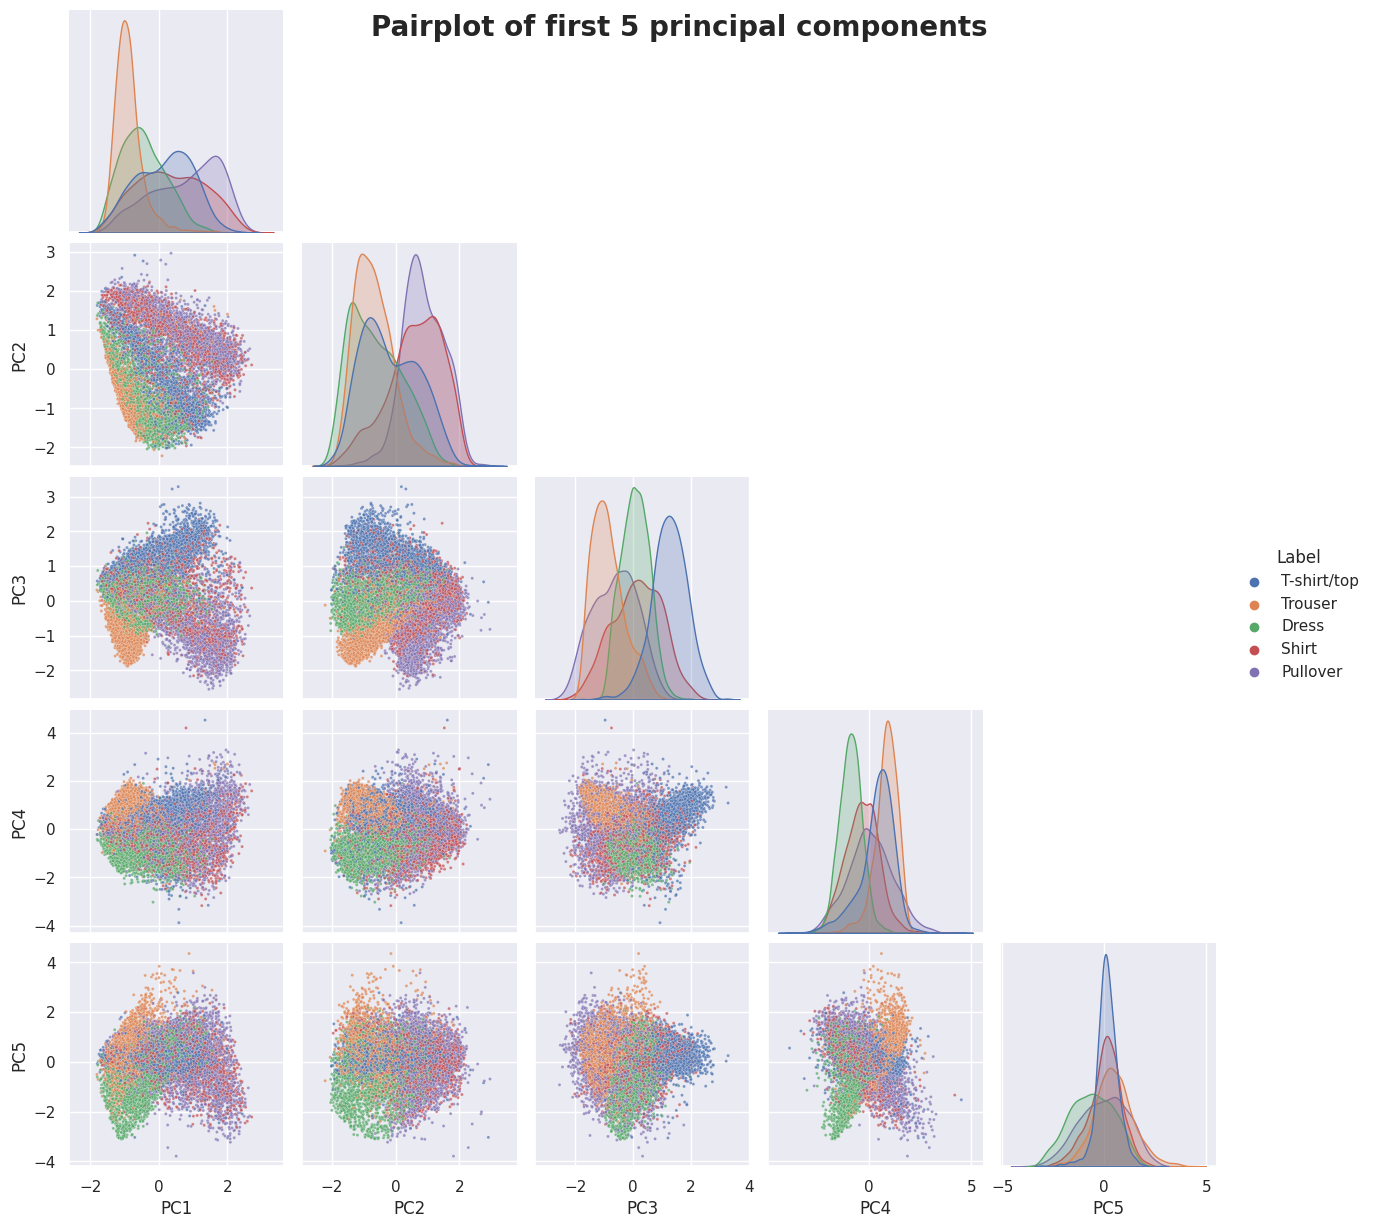
\includegraphics[width=1\textwidth]
    {images/pairplot_whitened_PCA.png}
    \caption{PCA pairplot}
\end{figure}

\newpage

\section{Backpropagation Python implementation}
\label{app:backprop-code}
The highlighted lines are where the partial derivatives w.r.t. the different parameters are derived.
Lines 11-15 are where the gradients of the loss function w.r.t. the weights and biases in the final (output) layer are calculated.
Lines 21-27 are where the gradients for each of the subsequent layers (that all have Leaky ReLU activation function and therefore same derivative) are calculated.

\begin{minted}[highlightlines={11-15,21-27},linenos]{python}
    def _backward(self, y_batch):
        """Computes a single backward pass all the way through the network. 
        Also updates the weights and biases.

        Parameters
        ----------
        y_batch : 2d ndarray
            array of one-hot encoded ground_truth labels
        """

        delta = self.activations[-1] - y_batch

        grad_bias = delta.sum(0)

        grad_weight = self.activations[-2].T @ delta

        grad_biases, grad_weights = [], []
        grad_weights.append(grad_weight)
        grad_biases.append(grad_bias)

        for i in range(2, len(self.layers) + 1):
            layer = self.layers[-i + 1]
            dzda = delta @ layer.weights.T
            delta = dzda * leaky_relu_der(self.sums[-i])

            grad_bias = delta.sum(0)
            grad_weight = self.activations[-i - 1].T @ delta
            grad_weights.append(grad_weight)
            grad_biases.append(grad_bias)

        # reverse the gradient lists so we can index them normally.
        grad_biases_rev = list(reversed(grad_biases))
        grad_weights_rev = list(reversed(grad_weights))

        for i in range(0, len(self.layers)):
            self.layers[i].weights -= self.learning_rate * grad_weights_rev[i]
            self.layers[i].biases -= self.learning_rate * grad_biases_rev[i]
\end{minted}

\end{appendices}

\end{document}